\chapter{MAGNIFICATION}
\label{chapter:magnification}
This chapter details the main contribution of this thesis work: the magnification effect generated by manipulating the distances for both the texture and the graph network. Subsection~\ref{section:texture_magnification} explains the process used in transforming the rendered FBO texture that the satellite images (Section~\ref{section:satellite_images}) and road network (Section~\ref{section:road_network}) both render to.

The requirements for this non-linear magnification of a texture include the ability to specify an inner and 
outer radius of magnification as well as a linear zoom factor. The program is intended to create a visual
effect such that the non-linear region between the inner and outer radii smoothly blends the regions of linear
zoom and base level magnification. The resulting function that accomplishes these goals should be easily
extensible to allow for multiple cursors interacting with the system at the same time. 

In performing magnification, we attempt to show more information to the users while ensuring that the data is still continuous. Some data loss will occur as regions become demagnified, but we attempt to minimize this as much as possible. As noted by Keahey and Robertson, our piecewise function should be continuous on its boundaries: the linear and non-linear functions should return the same value at the inner radius, and the non-linear function should return the input
value at the outer radius \cite{Keahey1996}.

A similar transformation is applied to the nodes and endpoints of line segments for the graph network. As mentioned previously in Chapter~\ref{chapter:intro}, most of the data in the graph network corresponds to
physical locations, so when the underlying satellite images get transformed by the texture magnification, the 
nodes and line segments must move accordingly. This process is explained in 
Subsection~\ref{section:graph_magnification}.

\section{Texture Magnification}
\label{section:texture_magnification}

To simulate magnification when dealing with rendering textures, we perform transformations the entire FBO texture
based on proximity to mouse cursors. Given three values, an inner radius, \emph{$r_0$}, an outer radius, 
\emph{$r_1$}, \emph{z}, a linear zoom factor, we construct two different formula for performing either a linear 
or non-linear magnification.

\begin{figure}[htp] \centering
    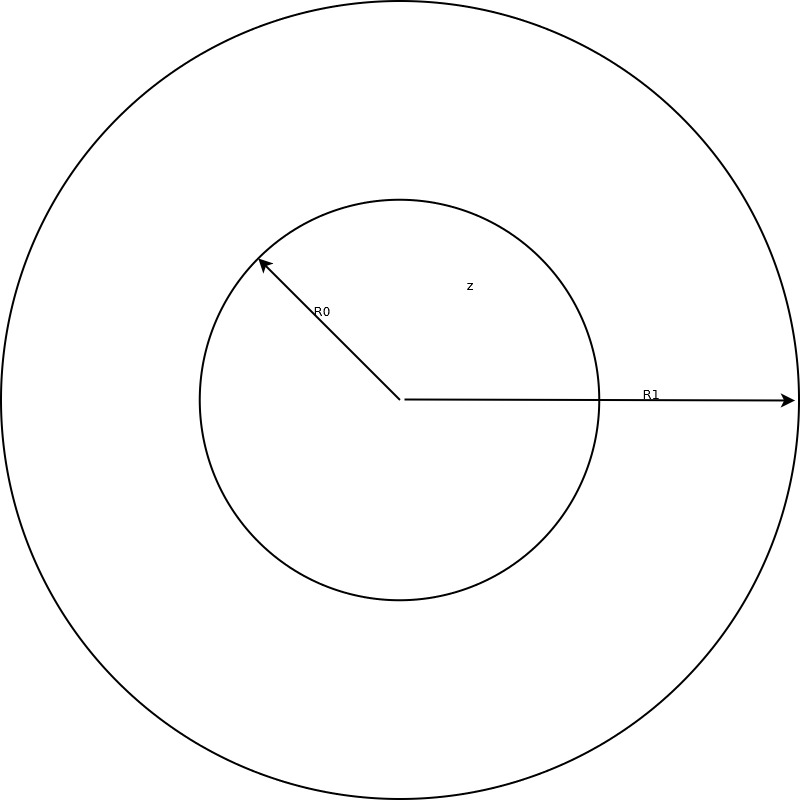
\includegraphics[width=0.4\linewidth]{img/cursor_mag.jpg}
    \caption[Magnification Parameters]{Visualization of the magnification parameters. \emph{z} is the linear zoom factor, \emph{$r_1$} is the outer radius, and \emph{$r_0$} is the inner radius.}
    \label{fig:mag_parameters}
\end{figure}

In both types of magnification, given the distance, \emph{d}, from a particular mouse cursor, $\vec{c}$,  to the 
original UV coordinate for a particular fragment, $\vec{p}$, the equations return a new scaled distance. This new 
distance, $f(d)$ is multiplied by the normalized direction vector between the mouse cursor, seen in
Equation~\ref{eq:magnifying_vector}.

\begin{equation}
    \label{eq:magnifying_vector} 
    v_i = f(d) \times \frac{\vec{c_i} - \vec{p}}{|\vec{c_i} - \vec{p}|}
\end{equation}

For distances less than \emph{$r_0$}, we perform linear magnification. The equation for which is given in 
Equation~\ref{eq:linear_magnification}

\begin{equation}
    \label{eq:linear_magnification}
    f(d) = d \times \frac{1}{z}
\end{equation}

We scale the distance by $\frac{1}{z}$ due to how UV sampling is performed. Reducing the area of the sampled 
texture spreads less information over the same area, resulting in the ability to see more data. An example of this is shown in Figure~\ref{fig:UV_sampling}.

\begin{figure}[htp] \centering
    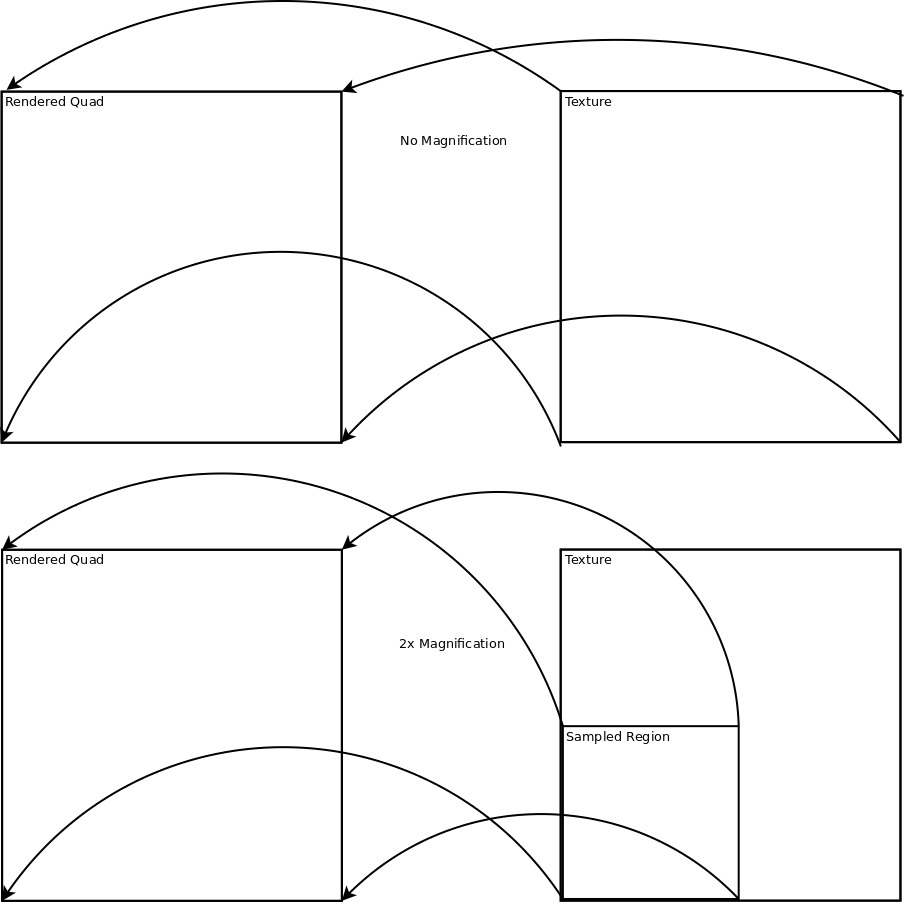
\includegraphics[width=0.6\linewidth]{img/texture_mag.jpg}
    \caption[UV Sampling]{Simple UV sampling example demonstrating magnification. The texture remains the same, we simply sample from a smaller region when performing magnification.}
    \label{fig:UV_sampling}
\end{figure}

For distances less than \emph{$r_1$}, we use the same premise of Equation~\ref{eq:linear_magnification}, but 
scale the linear zoom factor based on the distance away from the center instead of using a fixed value. To 
achieve this goal of a smooth, continuous image, we need a function which is continuous and has a smooth derivative. There are a few functions which follow the general form of having upper and lower limits; functions with a sigmoidal shape fall into this category. For our purposes, the desirable features are a smooth but rapid decrease from the higher magnification level, \emph{z} to the baseline level, 1. 
The generalized logistic function (Equation~\ref{eq:logistic_function}) fits these requirements as seen in 
Figure~\ref{fig:logistic_graph}, and is modified to fit our parameters, shown in 
Equation~\ref{eq:modified_logistic}

\begin{equation}
    \label{eq:logistic_function}
    f(x) = \frac{1}{1 + ae^{-bx}}
\end{equation}

\begin{equation}
    \label{eq:modified_logistic}
    f(d) = d \times \left( 1 + \epsilon + \frac{(z - 1 + 2\epsilon)}{1 + ae^{b(d-r_0)}}\right)
\end{equation}

The variables, \emph{a} and \emph{b}, can be solved for with the following two equations,~\ref{eq:solve_a} and~\ref{eq:solve_b}, essentially using a known given point to solve for the two variables.

\begin{equation}
    \label{eq:solve_a}
    a = \frac{\epsilon}{z - 1 + \epsilon}
\end{equation}

\begin{equation}
    \label{eq:solve_b}
    b = \frac{ln\left( \frac{\frac{z - 1 + 2 \epsilon }{\epsilon} + 1}{a}\right) }{r_1 - r_0}
\end{equation}

\begin{figure}[htp] \centering
    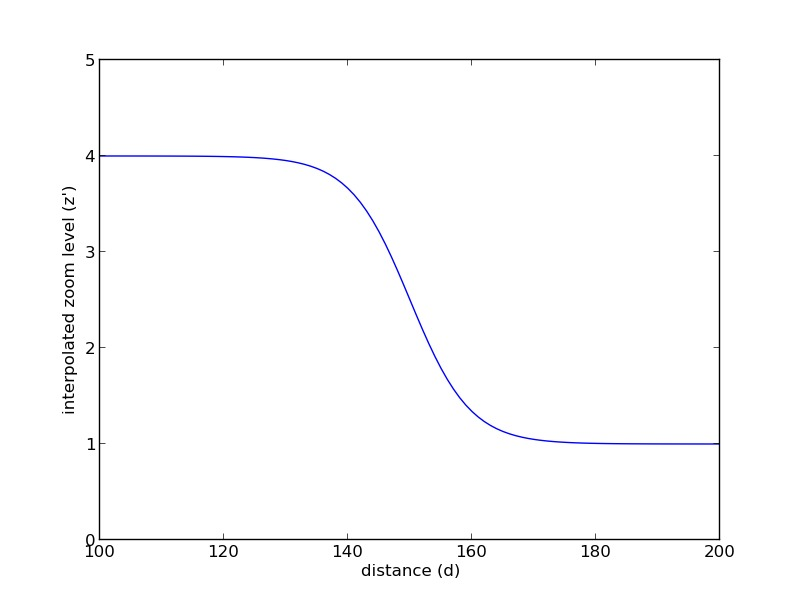
\includegraphics[width=0.8\linewidth]{img/logistic_graph.jpg}
    \caption[Logistic Graph]{Example graph of a logistic function with $\emph{$r_0$} = 100$, $\emph{$r_1$} = 200$, and $\emph{z} = 4$.}
    \label{fig:logistic_graph}
\end{figure}

The combined piecewise function for the distance function is shown below (Equation~\ref{eq:piecewise}).

\begin{equation}
    \label{eq:piecewise}
    f(d) = \left\{
        \begin{array}{lcr}
            d \times \frac{1}{z} & : & 0 < d < r_0 \\
            d \times \left( 1 + \epsilon + \frac{(z - 1 + 2\epsilon)}{1 + ae^{b(d-r_0)}}\right) & : & r_0 < d < r_1\\
            d & : & r_1 < d 
        \end{array}
    \right.
\end{equation}

A graph of the distances for the texture magnification functions is shown below in 
Figure~\ref{fig:texture_mag_graph} comparing the original distance and the computed distance.

\begin{figure}[htp] \centering
    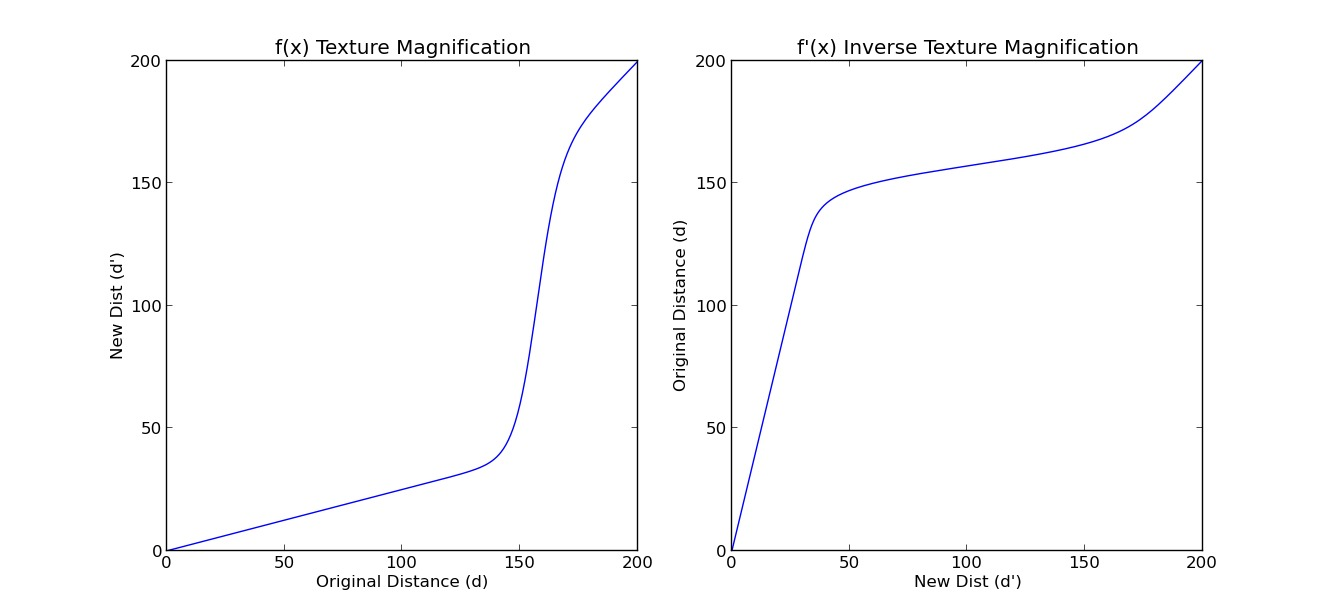
\includegraphics[width=0.8\linewidth]{img/full_graph.jpg}
    \caption[Distance Function]{Graph of the piecewise function, the x axis represents the original distance from 
    the mouse cursor and the y axis represents the new computed distance from the mouse cursor. The right image 
    is the graph of the inverse of the piecewise function. This figure shows that both functions have the same 
    domain and range.}
    \label{fig:texture_mag_graph}
\end{figure}

\section{Graph Magnification}
\label{section:graph_magnification}
To move the graph network correctly, we must use functions that are related to the texture magnification 
functions above. To perform magnification on a texture, we decrease the distance between the original UV coordinate and the focal point. If we decrease the distance between a cursor and a graph element, we cause the data to become clustered around the cursor instead of moving further away from the cursor.

Both functions map to the same domain and range. For any input between 0 and the outer radius, $r_1$, the output 
of the distance function should also be between 0 and $r_1$. The function for moving the graph network is also 
piecewise, much like the texture magnification functions.

If we examine the linear magnification function and its inverse for texture magnification, we can deduce that the correct way magnify the graph network is the 
inverse of the texture magnification function. The inverse of the linear magnification transformation (seen in 
Equation~\ref{eq:linear_magnification}) is trivial to compute, and is shown below in 
Equation~\ref{eq:inverse_linear_magnification}. The original function transforms values in the range of 0 to 
$r_0$ to 0 to $\frac{r_0}{z}$, so the inverse equation only accepts inputs in the range 0 to $\frac{r_0}{z}$.

\begin{equation}
    \label{eq:inverse_linear_magnification}
    g(d) = d \times {z}
\end{equation}

While the linear equation is trivial to invert, the logarithmic function is impractical to do analytically. The 
simplified version of the non-linear texture magnification is shown in Equation~\ref{eq:simple_log}. Solving this 
problem requires using Lambert W functions \cite{Corless1996}. Solving this equation was outside of the scope of the thesis, so we avoid solving this problem analytically by solving Equation~\ref{eq:modified_logistic} and storing the values in an 
array. Retrieving the values from the array uses a binary search to find the solution. For our purposes, we stored every value in the range from $r_0$ to $r_1$ with an interval of $0.1$. This interval was discovered by viewing the derivative of the texture magnification function.

\begin{equation}
    \label{eq:simple_log}
    f(d) = de^{d}
\end{equation}

The full piecewise function for graph magnification is seen below, $BinarySearch(z,d)$ corresponds to the index in the table given by performing a binary search of the table with a zoom level, \emph{z}, for a particular distance, \emph{d}. Because we only store values from $r_0$ to $r_1$, we add $r_0$ to this value to get the answer for the inverse of the non-linear function.

\begin{equation}
    \label{eq:inv_piecewise}
    g(d) = \left\{
        \begin{array}{lcr}
            d \times z & : & 0 < d < \frac{r_0}{z} \\
            BinarySearch(z,d) + r_0 & : & \frac{r_0}{z} < d < r_1\\
            d & : & r_1 < d 
        \end{array}
    \right.
\end{equation}


\section{Multi-cursor Magnification}
\label{section:multi_cursor}

The techniques described in the previous sections (Section~\ref{section:texture_magnification} and~\ref{section:graph_magnification}) are all applicable for
situations where only a single mouse cursor is applied within $r_1$ pixels of the cursor. The formulas 
described above are extensible and only need to be modified slightly for usage when multiple cursors affect
a fragment or graph element.

Intuitively, we would expect that cursors closer to a point should have more of an effect on the final
position of a fragment or graph element than cursors that are further away. This intuition leads to one possible
solution of performing a weighted average to get a final position.

Instead of simply returning a new distance from the texture and graph magnification functions 
(Equations~\ref{eq:piecewise} and~\ref{eq:inv_piecewise}), we have each function return two values, 
the original distance and the vector corresponding to the direction it would have been moved in. 

Because we want cursors that are closer to the element being affected to have a stronger influence, we
assign a higher weight to cursors that are closer, a full equation is seen below 
(Equation~\ref{eq:weighted_cursors}). It is important to note that the weights add up to 1.0, as we should not
move a point more than it can be transformed by the single application of the magnification equations.

\begin{figure}[htp] \centering
    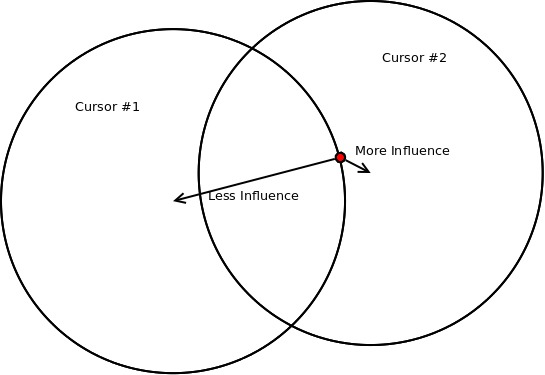
\includegraphics[width=0.6\linewidth]{img/multi_cursor.jpg}
    \caption[Multiple Cursor Magnification]{The two regions of magnification are seen overlapping a particular red point. Cursor 2 should have a higher weight when determining the final position, as it is closer to the original position of the point.}
    \label{fig:multi_cursor}
\end{figure}

\begin{equation}
    \label{eq:weighted_cursors}
    w_i = \frac{r_1 - d_i}{\sum\limits_{i=1}^n (r_1 - d_i)}
\end{equation}

\begin{equation}
    \label{eq:weighted_sum}
    \vec{v'} = \sum\limits_{i=1}^n w_i \vec{v_i}
\end{equation}

The vectors are multiplied by the corresponding weight, and the resulting vector is added to the original point
to get the new position of the element (Equation~\ref{eq:weighted_sum}). $\vec{v_i}$ the result of multiplying
the result of the piecewise function (Equation~\ref{eq:piecewise}) for texture magnification or graph manipulation
(Equation~\ref{eq:inv_piecewise}) by the normalized direction to the cursor $\vec{c_i}$.

\begin{figure}[htp] \centering
    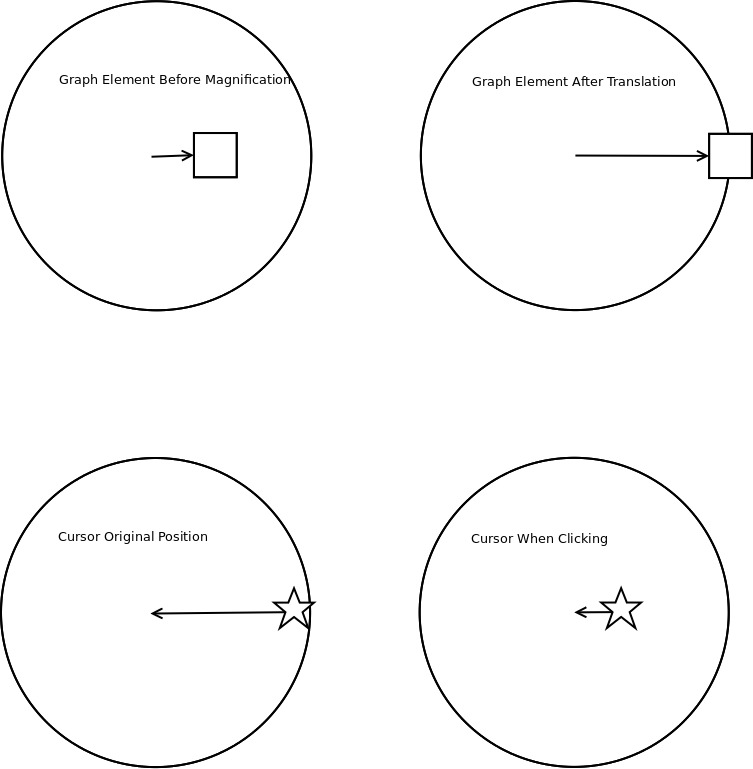
\includegraphics[width=0.6\linewidth]{img/clicking.jpg}
    \caption[Interacting with Magnified Elements]{The circular region represents the area magnified by a cursor at its center. The magnification that moves the graph element must be inverted to allow users to click on the actual position of the graph element, as seen in the bottom half of the image.}
    \label{fig:clicking}
\end{figure}

When interacting with the visualization application without magnification, every cursor is assumed to be directly over a point in screen space. However, when graph elements are moved due to being magnified by a cursor, we must compensate for the magnified position to interact with the node accordingly. Seen in Figure~\ref{fig:clicking}, we perform the texture magnification equations on a cursor to find the original position of a graph element. This occurs only when clicking on a graph
element, the cursor does not actually change its position on the screen.

\section{Summary}
\label{subsection:magnification_summary}

This chapter detailed the main magnification function used for our application for both satellite images and the graph network. A method for applying this function when multiple points of focus are included is also described. The following chapter discusses the application's overall performance and a short survey of responses to the new system.
